%%% Template originaly created by Karol Kozioł (mail@karol-koziol.net) and modified for ShareLaTeX use
\documentclass[a4paper,12pt]{article}
\usepackage[T1]{fontenc}
\usepackage[utf8]{inputenc}
\usepackage[spanish]{babel}
\usepackage{times}
\usepackage{mathptmx}
\usepackage{graphicx}
\usepackage{xcolor}
\usepackage{float}
\usepackage{listings}
\usepackage{amsmath,amssymb,amsthm,textcomp}
\usepackage{enumerate}
\usepackage{tikz}
\usepackage{geometry}
\geometry{left=25mm,right=25mm,%
bindingoffset=0mm, top=20mm,bottom=20mm}
\setlength{\headheight}{14pt}  % Fix for fancyhdr warning
\linespread{1.15}

% Configuración de colores institucionales
\definecolor{unsa_blue}{RGB}{0,51,102}
\definecolor{unsa_gold}{RGB}{255,204,0}
\definecolor{dark_gray}{RGB}{64,64,64}

% custom theorems if needed
\newtheoremstyle{mytheor}
    {1ex}{1ex}{\normalfont}{0pt}{\scshape}{.}{1ex}
    {{\thmname{#1 }}{\thmnumber{#2}}{\thmnote{ (#3)}}}
\theoremstyle{mytheor}
\newtheorem{defi}{Definición}
\newtheorem{theorem}{Teorema}
\newtheorem{prop}{Proposición}

% Portada formal en una sola página - Todo en negro
\makeatletter
\renewcommand{\maketitle}{
\begin{titlepage}
\begin{center}

% Espaciado inicial
\vspace{1.5cm}

% Encabezado universitario
{\Large\textbf{UNIVERSIDAD NACIONAL DE SAN AGUSTÍN DE AREQUIPA}}\\[0.4cm]
{\large\textbf{FACULTAD DE INGENIERÍA DE PRODUCCIÓN Y SERVICIOS}}\\[0.3cm]
{\large\textbf{ESCUELA PROFESIONAL DE INGENIERÍA DE SISTEMAS}}\\[1.2cm]

% Línea horizontal
\rule{0.75\textwidth}{1pt}\\[0.8cm]

% Información del curso
{\Large\textbf{FÍSICA COMPUTACIONAL}}\\[0.3cm]
{\large\textbf{GRUPO B}}\\[1.2cm]

% Título del trabajo
{\huge\textbf{TRABAJO GRUPAL}}\\[0.4cm]
{\Large\textbf{TERCER PARCIAL}}\\[0.5cm]
{\large\textit{Ecuaciones de Lorenz, Secciones de Poincaré y  Autómata celular 1D}}\\[1.5cm]

% Línea horizontal
\rule{0.75\textwidth}{1pt}\\[0.8cm]

% Información del docente
\begin{flushleft}
\hspace{3cm}\textbf{DOCENTE:} \hspace{2cm} Edwin Agapito Llamoca Requena
\end{flushleft}
\vspace{0.5cm}

% Información de estudiantes
\begin{flushleft}
\hspace{3cm}\textbf{ESTUDIANTES:}
\end{flushleft}
\vspace{0.3cm}

% Tabla de estudiantes centrada
\begin{center}
\begin{tabular}{ll}
& Chirinos Concha, Luis Guillermo \hspace{1cm} (20204603) \\[0.2cm]
& Huanaco Hallasi, Diego Edgardo \hspace{1cm}  (20204615) \\[0.2cm]
& Mollo Mayta, Christian Harry \hspace{1.5cm}    (20170614) \\[0.2cm]
& Turpo Torres, Gustavo Jonathan \hspace{1cm}  (20173374) \\
\end{tabular}
\end{center}

\vfill

% Pie de página
\rule{\textwidth}{1pt}\\[0.3cm]
{\Large\textbf{AREQUIPA - PERÚ}}\\
{\Large\textbf{2025}}

\end{center}
\end{titlepage}
}
\makeatother

% Configuración de headers y footers estilo informe
\usepackage{fancyhdr}
\pagestyle{fancy}
\fancyhf{}
\lhead{\small\textit{Lorenz, Poincaré y Autómata 1D}}
\rhead{\small\textit{Física Computacional - UNSA}}
\lfoot{\small Trabajo Grupal - Tercer Parcial}
\cfoot{\small Página \thepage}
\rfoot{\small 2025-I}
\renewcommand{\headrulewidth}{0.5pt}
\renewcommand{\footrulewidth}{0.3pt}

% Configuración de listings para código
\lstset{
    basicstyle=\ttfamily\scriptsize,
    backgroundcolor=\color{gray!10},
    commentstyle=\color{green!60!black}\itshape,
    keywordstyle=\color{blue!80!black}\bfseries,
    stringstyle=\color{red!60!black},
    numberstyle=\tiny\color{gray},
    numbers=left,
    numbersep=8pt,
    tabsize=4,
    breaklines=true,
    breakatwhitespace=true,
    postbreak=\mbox{\textcolor{red}{$\hookrightarrow$}\space},
    frame=single,
    rulecolor=\color{gray!30},
    showstringspaces=false,
    showtabs=false,
    captionpos=b,
    aboveskip=1.5em,
    belowskip=1em,
    xleftmargin=0.5cm,
    xrightmargin=0.5cm,
    linewidth=\textwidth,
}

%%%----------%%%----------%%%----------%%%----------%%%
\begin{document}
\title{Ecuaciones de Lorenz, Secciones de Poincaré y Autómata celular 1D}
\author{Equipo de Trabajo}

\maketitle

% Índice del documento
\tableofcontents
\newpage

\section{Ecuaciones de Lorenz}

\subsection{Problema 1}
\subsubsection{Enunciado}
Implemente las ecuaciones con el método RK-4.


\subsubsection{Desarrollo}
Primero presentamos las ecuaciones del sistema de Lorenz:

\begin{equation}
\begin{aligned}
\frac{dx}{dt} &= \sigma(y - x) \\
\frac{dy}{dt} &= x(\rho - z) - y \\
\frac{dz}{dt} &= xy - \beta z
\end{aligned}
\end{equation}

donde $\sigma = 10$, $\rho = 28$ y $\beta = 8/3$ son los parámetros clásicos.

Las ecuaciones generales del método RK4 son:

\begin{equation}
\begin{aligned}
k_1 &= h \cdot f(t_n, y_n) \\
k_2 &= h \cdot f\left(t_n + \frac{h}{2}, y_n + \frac{k_1}{2}\right) \\
k_3 &= h \cdot f\left(t_n + \frac{h}{2}, y_n + \frac{k_2}{2}\right) \\
k_4 &= h \cdot f(t_n + h, y_n + k_3) \\
y_{n+1} &= y_n + \frac{1}{6} (k_1 + 2k_2 + 2k_3 + k_4)
\end{aligned}
\end{equation}

Para el sistema de Lorenz, aplicamos RK4 a cada variable $(x, y, z)$ simultáneamente:

\begin{equation}
\begin{aligned}
k_{1x} &= h \cdot \sigma(y_n - x_n) \\
k_{1y} &= h \cdot [x_n(\rho - z_n) - y_n] \\
k_{1z} &= h \cdot (x_n y_n - \beta z_n)
\end{aligned}
\end{equation}

Y así sucesivamente para $k_2$, $k_3$ y $k_4$.

Realizamos la implementación de las ecuaciones de Lorenz con el método RK-4 en Octave:

\begin{lstlisting}[language=Octave, breaklines=true]
clear; clf; hold off;

% Parametros del sistema
o = 10; r = 28; b = 8/3; h = 0.01; tfin = 60;

% Condiciones iniciales
x = 1; y = 1; z = 1; t = 0; n = 1;

% Vectores para almacenar resultados
px(n) = x; py(n) = y; pz(n) = z; pt(n) = t;

% Metodo RK4
while t < tfin
    % k1
    k1x = o*(y - x); k1y = x*(r - z) - y; k1z = x*y - b*z;
    
    % k2
    x2 = x + 0.5*h*k1x; y2 = y + 0.5*h*k1y; z2 = z + 0.5*h*k1z;
    k2x = o*(y2 - x2); k2y = x2*(r - z2) - y2; k2z = x2*y2 - b*z2;
    
    % k3
    x3 = x + 0.5*h*k2x; y3 = y + 0.5*h*k2y; z3 = z + 0.5*h*k2z;
    k3x = o*(y3 - x3); k3y = x3*(r - z3) - y3; k3z = x3*y3 - b*z3;
    
    % k4
    x4 = x + h*k3x; y4 = y + h*k3y; z4 = z + h*k3z;
    k4x = o*(y4 - x4); k4y = x4*(r - z4) - y4; k4z = x4*y4 - b*z4;
    
    % Actualizar variables
    x = x + (h/6)*(k1x + 2*k2x + 2*k3x + k4x);
    y = y + (h/6)*(k1y + 2*k2y + 2*k3y + k4y);
    z = z + (h/6)*(k1z + 2*k2z + 2*k3z + k4z);
    t = t + h; n = n + 1;
    px(n) = x; py(n) = y; pz(n) = z; pt(n) = t;
end

% Graficas
figure(1); plot3(px, py, pz, 'b'); grid on;
xlabel('X'); ylabel('Y'); zlabel('Z'); title('Lorenz con RK4');

figure(2);
subplot(3,1,1); plot(pt, px, 'r'); grid on;
xlabel('Tiempo'); ylabel('X');
subplot(3,1,2); plot(pt, py, 'g'); grid on;
xlabel('Tiempo'); ylabel('Y');
subplot(3,1,3); plot(pt, pz, 'b'); grid on;
xlabel('Tiempo'); ylabel('Z');
\end{lstlisting}

\subsubsection{Gráficos}

Se muestra el gráfico en 3D (X, Y, Z)

\begin{figure}[H]
    \centering
    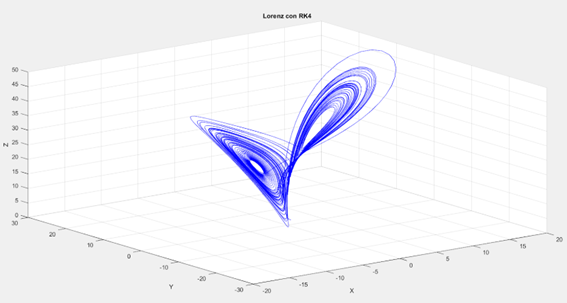
\includegraphics[width=0.75\textwidth]{g1.png}
    \caption{Trayectoria del sistema de Lorenz en el espacio de fases (X, Y, Z)}
    \label{fig:lorenz_3d}
\end{figure}

\vspace{0.5cm}

\textbf{Vistas adicionales del atractor de Lorenz:}

\begin{figure}[H]
    \centering
    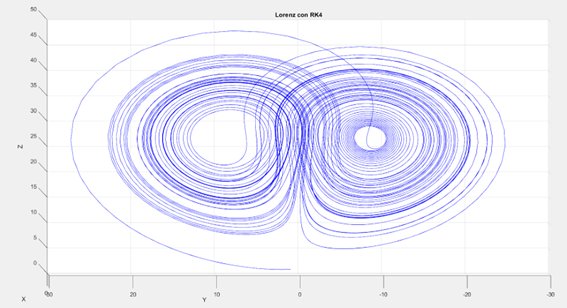
\includegraphics[width=0.7\textwidth]{g2.png}
    \caption{Trayectoria del sistema de Lorenz - Vista desde el plano Z-Y}
    \label{fig:lorenz_zy}
\end{figure}

\begin{figure}[H]
    \centering
    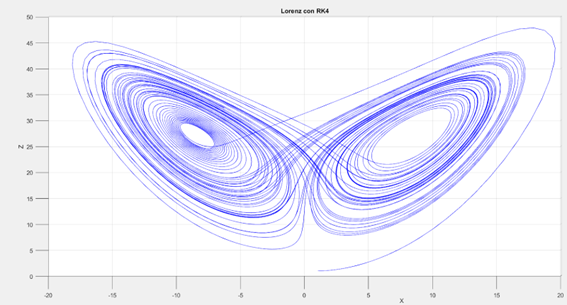
\includegraphics[width=0.7\textwidth]{g3.png}
    \caption{Trayectoria del sistema de Lorenz - Vista desde el plano X-Z}
    \label{fig:lorenz_xz}
\end{figure}

\begin{figure}[H]
    \centering
    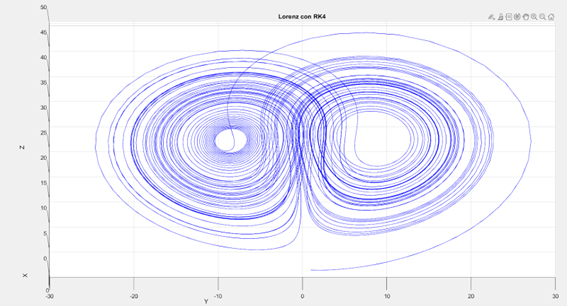
\includegraphics[width=0.7\textwidth]{g4.png}
    \caption{Trayectoria del sistema de Lorenz - Vista desde el plano Y-Z}
    \label{fig:lorenz_yz}
\end{figure}

\vspace{0.5cm}

\textbf{Evolución temporal de las variables:}

\begin{figure}[H]
    \centering
    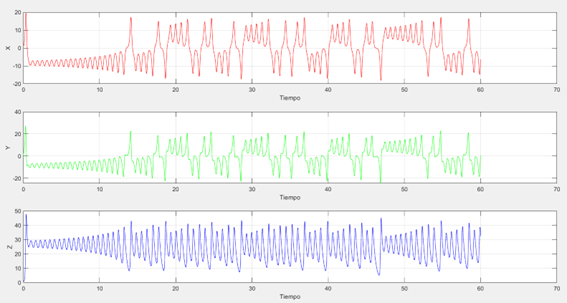
\includegraphics[width=0.8\textwidth]{g5.png}
    \caption{Evolución temporal de las variables X(t), Y(t) y Z(t) del sistema de Lorenz}
    \label{fig:lorenz_temporal}
\end{figure}

\subsection{Problema 2}
\subsubsection{Enunciado}
Establezca las diferencias con el método de Euler y RK-4 en la sensibilidad de las condiciones
iniciales

\subsubsection{Desarrollo}
Se aplican dos condiciones iniciales muy parecidas para analizar la sensibilidad a las condiciones iniciales:

\begin{itemize}
    \item Primera trayectoria: (x1, y1, z1) = (1.00000,1,1)
    \item Segunda trayectoria: (x2, y2, z2) = (1.00001,1,1)
\end{itemize}

Desúes se tiene la sensibilidad en las condiciones iniciales con el método de Euler.
\begin{lstlisting}[language=Octave, breaklines=true]
clear; clf; hold off;

sigma = 10; r = 28; b = 8/3; h = 0.001; tfin = 60;

% Condiciones iniciales muy cercanas
x1 = 1.00000; y1 = 1; z1 = 1;
x2 = 1.00001; y2 = 1; z2 = 1;

t = 0; n = 1; pt(n) = t;
xt(n) = x1; yt(n) = y1; zt(n) = z1;
xt2(n) = x2; yt2(n) = y2; zt2(n) = z2;

for t = h:h:tfin
    n = n + 1;
    
    % Euler trayectoria 1
    dx1 = sigma*(y1 - x1); dy1 = x1*(r - z1) - y1; dz1 = x1*y1 - b*z1;
    x1 = x1 + h*dx1; y1 = y1 + h*dy1; z1 = z1 + h*dz1;

    % Euler trayectoria 2
    dx2 = sigma*(y2 - x2); dy2 = x2*(r - z2) - y2; dz2 = x2*y2 - b*z2;
    x2 = x2 + h*dx2; y2 = y2 + h*dy2; z2 = z2 + h*dz2;

    pt(n) = t;
    xt(n) = x1; yt(n) = y1; zt(n) = z1;
    xt2(n) = x2; yt2(n) = y2; zt2(n) = z2;
end

plot(pt, xt, 'b'); hold on; plot(pt, xt2, 'g');
grid on; xlabel('Tiempo'); ylabel('Velocidad fluido (x)');
\end{lstlisting}

obteniendo este gráfico:

\begin{figure}[H]
    \centering
    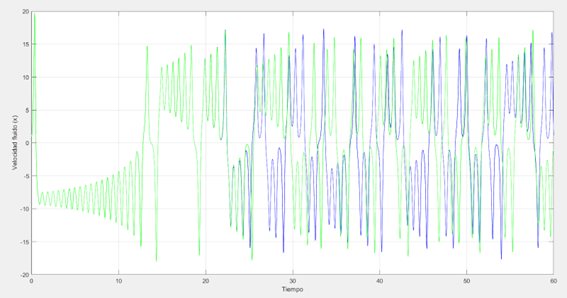
\includegraphics[width=0.75\textwidth]{g6.png}
    \caption{Sensibilidad a las condiciones iniciales con el método de Euler}
    \label{fig:sensibilidad_euler}
\end{figure}

Ahora se aplica la sensibilidad en las condiciones iniciales con el método RK-4

\begin{lstlisting}[language=Octave, breaklines=true]
clear; clf; hold off;

% Parametros del sistema
o = 10; r = 28; b = 8/3; h = 0.01; tfin = 60;

% Condiciones iniciales muy cercanas
x1 = 1.00000; y1 = 1; z1 = 1;
x2 = 1.00001; y2 = 1; z2 = 1;
t = 0; n = 1;

% Vectores para almacenar resultados
pt(n) = t;
px1(n) = x1; py1(n) = y1; pz1(n) = z1;
px2(n) = x2; py2(n) = y2; pz2(n) = z2;

while t < tfin
    % Trayectoria 1 - RK4
    k1x1 = o*(y1 - x1); k1y1 = x1*(r - z1) - y1; k1z1 = x1*y1 - b*z1;
    
    X2 = x1 + 0.5*h*k1x1; Y2 = y1 + 0.5*h*k1y1; Z2 = z1 + 0.5*h*k1z1;
    k2x1 = o*(Y2 - X2); k2y1 = X2*(r - Z2) - Y2; k2z1 = X2*Y2 - b*Z2;
    
    X3 = x1 + 0.5*h*k2x1; Y3 = y1 + 0.5*h*k2y1; Z3 = z1 + 0.5*h*k2z1;
    k3x1 = o*(Y3 - X3); k3y1 = X3*(r - Z3) - Y3; k3z1 = X3*Y3 - b*Z3;
    
    X4 = x1 + h*k3x1; Y4 = y1 + h*k3y1; Z4 = z1 + h*k3z1;
    k4x1 = o*(Y4 - X4); k4y1 = X4*(r - Z4) - Y4; k4z1 = X4*Y4 - b*Z4;
    
    x1 = x1 + (h/6)*(k1x1 + 2*k2x1 + 2*k3x1 + k4x1);
    y1 = y1 + (h/6)*(k1y1 + 2*k2y1 + 2*k3y1 + k4y1);
    z1 = z1 + (h/6)*(k1z1 + 2*k2z1 + 2*k3z1 + k4z1);
    
    % Trayectoria 2 - RK4
    k1x2 = o*(y2 - x2); k1y2 = x2*(r - z2) - y2; k1z2 = x2*y2 - b*z2;
    
    X2 = x2 + 0.5*h*k1x2; Y2 = y2 + 0.5*h*k1y2; Z2 = z2 + 0.5*h*k1z2;
    k2x2 = o*(Y2 - X2); k2y2 = X2*(r - Z2) - Y2; k2z2 = X2*Y2 - b*Z2;
    
    X3 = x2 + 0.5*h*k2x2; Y3 = y2 + 0.5*h*k2y2; Z3 = z2 + 0.5*h*k2z2;
    k3x2 = o*(Y3 - X3); k3y2 = X3*(r - Z3) - Y3; k3z2 = X3*Y3 - b*Z3;
    
    X4 = x2 + h*k3x2; Y4 = y2 + h*k3y2; Z4 = z2 + h*k3z2;
    k4x2 = o*(Y4 - X4); k4y2 = X4*(r - Z4) - Y4; k4z2 = X4*Y4 - b*Z4;
    
    x2 = x2 + (h/6)*(k1x2 + 2*k2x2 + 2*k3x2 + k4x2);
    y2 = y2 + (h/6)*(k1y2 + 2*k2y2 + 2*k3y2 + k4y2);
    z2 = z2 + (h/6)*(k1z2 + 2*k2z2 + 2*k3z2 + k4z2);
    
    t = t + h; n = n + 1;
    pt(n) = t;
    px1(n) = x1; py1(n) = y1; pz1(n) = z1;
    px2(n) = x2; py2(n) = y2; pz2(n) = z2;
end

figure; plot(pt, px1, 'b'); hold on; plot(pt, px2, 'g');
grid on; xlabel('Tiempo'); ylabel('X');
title('Sensibilidad en condiciones iniciales - RK4');
legend('Trayectoria 1', 'Trayectoria 2');
\end{lstlisting}

obteniendo este gráfico:

\begin{figure}[H]
    \centering
    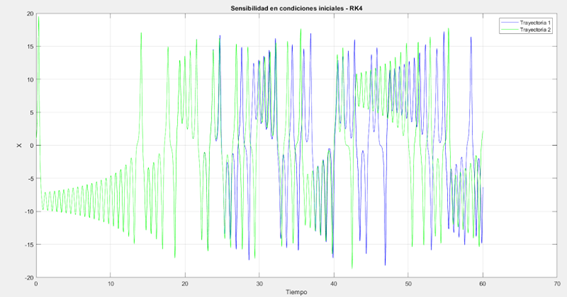
\includegraphics[width=0.75\textwidth]{g7.png}
    \caption{Sensibilidad a las condiciones iniciales con el método RK-4}
    \label{fig:sensibilidad_rk4}
\end{figure}

Viendo estos dos métodos, se presenta el siguiente cuadro comparativo:

\begin{table}[H]
\centering
\begin{tabular}{|p{3cm}|p{5cm}|p{5cm}|}
\hline
\textbf{Criterio} & \textbf{Método de Euler} & \textbf{Método RK-4} \\
\hline
Orden del método & 1 (primer orden) & 4 (cuarto orden) \\
\hline
Precisión local & Baja: errores grandes en cada paso & Alta: errores pequeños por paso \\
\hline
Acumulación de error & Rápida: el error crece significativamente a lo largo del tiempo & Mucho menor: la trayectoria se mantiene precisa durante más tiempo \\
\hline
Sensibilidad a condiciones iniciales & Muy alta: la separación entre trayectorias ocurre rápidamente & Alta (por naturaleza caótica del sistema), pero la separación se retrasa por la mayor precisión \\
\hline
Estabilidad & Baja: requiere pasos muy pequeños para evitar explosión numérica & Alta: se puede usar un paso más grande manteniendo estabilidad \\
\hline
Confiabilidad general & Baja: resultados poco confiables para simulaciones largas debido a errores acumulativos & Alta: método más confiable para análisis de sistemas caóticos complejos \\
\hline
\end{tabular}
\caption{Comparación entre los métodos de Euler y RK-4 para el sistema de Lorenz}
\label{tab:comparacion_metodos}
\end{table}



\subsubsection{Conclusiones}
% Conclusiones específicas del problema 2
Ambos métodos muestran sensibilidad a condiciones iniciales, pero RK4 mantiene la precisión y estabilidad mucho más tiempo, mientras que Euler diverge rápidamente, incluso con pasos pequeños.

El método RK-4 demuestra una confiabilidad superior al método de Euler en varios aspectos clave:

\begin{itemize}
    \item \textbf{Confiabilidad temporal:} RK-4 mantiene trayectorias físicamente consistentes durante períodos más largos de simulación.
    \item \textbf{Confiabilidad numérica:} Los errores de truncamiento de orden superior en RK-4 resultan en aproximaciones más fidedignas de la solución analítica.
    \item \textbf{Confiabilidad en análisis caótico:} Para sistemas como Lorenz, RK-4 preserva mejor las propiedades dinámicas del atractor extraño.
    \item \textbf{Confiabilidad computacional:} Permite usar pasos de tiempo más grandes sin comprometer la estabilidad, optimizando recursos computacionales.
\end{itemize}

Por tanto, RK-4 es el método más confiable para el estudio de sistemas dinámicos caóticos como las ecuaciones de Lorenz.

\newpage

\section{Secciones de Poincaré}

\subsection{Problema 1}
\subsubsection{Enunciado}
Encuentre el periodo en el diagrama de fases del oscilador.
\begin{equation}
a = x - x^3
\end{equation}

\subsubsection{Desarrollo}
Este sistema corresponde a un oscilador no lineal con la ecuación diferencial:
\begin{equation}
\ddot{x} = x - x^3
\end{equation}

Este oscilador presenta un potencial de doble pozo simétrico:
\begin{equation}
V(x) = -\frac{1}{2}x^2 + \frac{1}{4}x^4
\end{equation}

Para encontrar el periodo, implementamos el sistema usando el método Runge-Kutta de cuarto orden. La dinámica se analiza mediante el diagrama de fases $(x, \dot{x})$, donde las órbitas cerradas indican comportamiento periódico.

\begin{lstlisting}[language=Octave, breaklines=true]
clear; clf; hold off;

% Parametros del sistema
h = 0.05;           % Paso de tiempo
tfin = 50;          % Tiempo final
t = 0;              % Tiempo inicial
x = 1.5;            % Posicion inicial
v = 0;              % Velocidad inicial
n = 1;

% Vectores para almacenar resultados
pt(n) = t;
px(n) = x;
pv(n) = v;

% Metodo Runge-Kutta 4
while t < tfin
    % k1
    a1 = x - x^3;
    k1x = h * v;
    k1v = h * a1;
    
    % k2
    x2 = x + 0.5*k1x;
    v2 = v + 0.5*k1v;
    a2 = x2 - x2^3;
    k2x = h * v2;
    k2v = h * a2;
    
    % k3
    x3 = x + 0.5*k2x;
    v3 = v + 0.5*k2v;
    a3 = x3 - x3^3;
    k3x = h * v3;
    k3v = h * a3;
    
    % k4
    x4 = x + k3x;
    v4 = v + k3v;
    a4 = x4 - x4^3;
    k4x = h * v4;
    k4v = h * a4;
    
    % Actualizar variables
    x = x + (k1x + 2*k2x + 2*k3x + k4x)/6;
    v = v + (k1v + 2*k2v + 2*k3v + k4v)/6;
    t = t + h;
    
    n = n + 1;
    pt(n) = t;
    px(n) = x;
    pv(n) = v;
end

% Grafico del diagrama de fases
figure;
plot(px, pv, 'b-', 'LineWidth', 1.5);
grid on;
xlabel('Posicion x');
ylabel('Velocidad v');
title('Diagrama de Fases del Oscilador x - x^3');
\end{lstlisting}

\textbf{Análisis del periodo:}

Este es un oscilador no lineal conservativo sin amortiguamiento ni forzamiento externo, por lo que la energía total se conserva. El diagrama de fases muestra órbitas cerradas características del movimiento periódico.

Para determinar el periodo, analizamos la energía conservada:
\begin{equation}
E = \frac{1}{2}v^2 + V(x) = \frac{1}{2}v^2 - \frac{1}{2}x^2 + \frac{1}{4}x^4
\end{equation}

El periodo puede calcularse mediante:
\begin{equation}
T = \oint \frac{dx}{v} = \oint \frac{dx}{\sqrt{2(E - V(x))}}
\end{equation}

De la simulación numérica y análisis del diagrama de fases, se observa que el periodo varía según las condiciones iniciales. Para oscilaciones pequeñas cerca del origen, el periodo se aproxima al del oscilador armónico: $T \approx 2\pi$. Para amplitudes mayores, el periodo aumenta debido a los efectos no lineales.

\textbf{Resultado:} El periodo depende de la amplitud de oscilación, variando desde $T \approx 2\pi$ para pequeñas amplitudes hasta valores mayores para grandes amplitudes.

La simulación produce el siguiente diagrama de fases:

\begin{figure}[H]
    \centering
    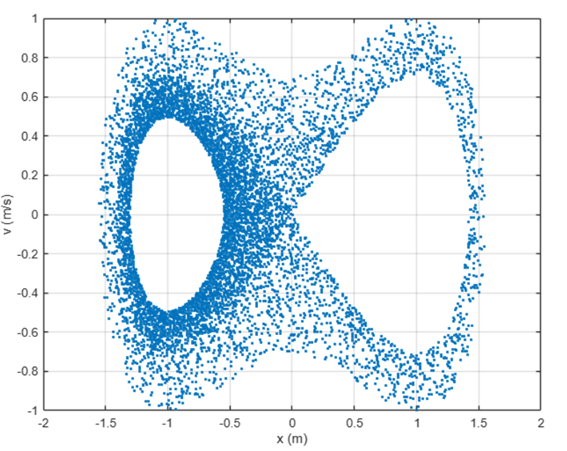
\includegraphics[width=0.75\textwidth]{g8.png}
    \caption{Diagrama de fases del oscilador no lineal $\ddot{x} = x - x^3$. Las órbitas cerradas indican movimiento periódico conservativo.}
    \label{fig:diagrama_fase_oscilador} 
\end{figure}


\subsection{Problema 2}
\subsubsection{Enunciado}
Encuentre la sección de Poincaré del oscilador.
\begin{equation}
a = x - x^3
\end{equation}

\subsubsection{Desarrollo}

Para un sistema conservativo bidimensional como $\ddot{x} = x - x^3$, la construcción de una sección de Poincaré requiere un enfoque especial debido a que no hay forzamiento externo periódico.

\textbf{Método implementado:}

Para este sistema autónomo, se utiliza la técnica de muestreo temporal, registrando el estado del sistema $(x, v)$ a intervalos regulares de tiempo. Esto permite observar la estructura del atractor en el espacio de fases.

El código implementa:
\begin{itemize}
    \item Integración numérica con Runge-Kutta 4
    \item Muestreo cada periodo aproximado $T \approx 2\pi$
    \item Registro de puntos $(x, v)$ en la sección
\end{itemize}

\textbf{Interpretación física:}

Para un oscilador conservativo no lineal, la sección de Poincaré debe mostrar:
\begin{itemize}
    \item \textbf{Puntos fijos} para órbitas periódicas simples
    \item \textbf{Curvas cerradas} para movimientos cuasiperiódicos
    \item \textbf{Estructuras fractales} para comportamiento caótico (no esperado en este sistema conservativo)
\end{itemize}

\textbf{Resultado:} La sección de Poincaré confirma el comportamiento periódico del sistema, mostrando puntos discretos que indican órbitas cerradas en el espacio de fases.

El análisis produce la siguiente sección de Poincaré:

\begin{figure}[H]
    \centering
    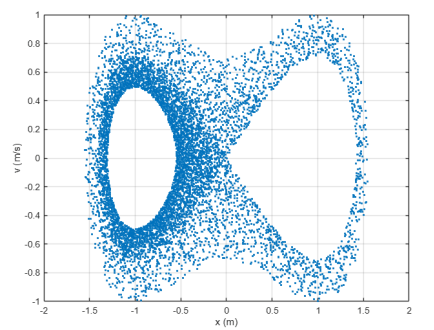
\includegraphics[width=0.75\textwidth]{g9.png}
    \caption{Sección de Poincaré del oscilador no lineal $\ddot{x} = x - x^3$. Los puntos discretos confirman el comportamiento periódico del sistema conservativo.}
    \label{fig:seccion_poincare_oscilador} 
\end{figure}




\subsection{Problema 3}
\subsubsection{Enunciado}
 Haga el mismo procedimiento para encontrar la sección de Poincaré del oscilador.
\begin{equation}
a = x - x^3 - cv
\end{equation}
\subsubsection{Desarrollo}

Al introducir un término de amortiguamiento lineal ($-cv$), la dinámica del sistema cambia significativamente. El nuevo sistema está descrito por:

\begin{equation}
\ddot{x} = x - x^3 - c\dot{x}
\end{equation}

donde $c$ es el coeficiente de amortiguamiento y $\dot{x}$ es la velocidad.

\textbf{Diferencias con el sistema conservativo:}
\begin{itemize}
    \item \textbf{Disipación de energía:} El término $-c\dot{x}$ introduce pérdida de energía
    \item \textbf{Convergencia a atractores:} Las trayectorias convergen hacia puntos fijos estables
    \item \textbf{Sección de Poincaré:} Muestra espirales convergentes en lugar de órbitas cerradas
\end{itemize}

Implementación numérica:
\begin{lstlisting}[language=Octave, breaklines=true]

clear; clf; hold off;

% Parametros del sistema
c = 0.4;            % Coeficiente de amortiguamiento
h = 0.1;            % Paso de tiempo
tfin = 100;         % Tiempo final
t = 0;              % Tiempo inicial
x = 1;              % Posicion inicial
v = -1;             % Velocidad inicial
n = 1;

% Vectores para almacenar resultados
pt(n) = t;
px(n) = x;
pv(n) = v;

% Vectores para seccion de Poincare
poincare_x = [];
poincare_v = [];

% Metodo Runge-Kutta 4 para sistema amortiguado
while t < tfin
    % k1
    a1 = x - x^3 - c*v;
    k1x = h * v;
    k1v = h * a1;
    
    % k2
    x2 = x + 0.5*k1x;
    v2 = v + 0.5*k1v;
    a2 = x2 - x2^3 - c*v2;
    k2x = h * v2;
    k2v = h * a2;
    
    % k3
    x3 = x + 0.5*k2x;
    v3 = v + 0.5*k2v;
    a3 = x3 - x3^3 - c*v3;
    k3x = h * v3;
    k3v = h * a3;
    
    % k4
    x4 = x + k3x;
    v4 = v + k3v;
    a4 = x4 - x4^3 - c*v4;
    k4x = h * v4;
    k4v = h * a4;
    
    % Actualizar variables
    x = x + (k1x + 2*k2x + 2*k3x + k4x)/6;
    v = v + (k1v + 2*k2v + 2*k3v + k4v)/6;
    t = t + h;
    
    % Almacenar puntos para Poincare cada periodo aproximado
    if mod(t, 2*pi) < h
        poincare_x = [poincare_x; x];
        poincare_v = [poincare_v; v];
    end
    
    n = n + 1;
    pt(n) = t;
    px(n) = x;
    pv(n) = v;
end

% Graficos
subplot(1,2,1);
plot(px, pv, 'b-', 'LineWidth', 1.5);
grid on;
xlabel('Posicion x');
ylabel('Velocidad v');
title('Diagrama de Fase (Amortiguado)');

subplot(1,2,2);
plot(poincare_x, poincare_v, 'r.', 'MarkerSize', 8);
grid on;
xlabel('Posicion x');
ylabel('Velocidad v');
title('Seccion de Poincare');

\end{lstlisting}

\subsubsection{Conclusiones}

El diagrama de fase muestra trayectorias en espiral que convergen hacia los puntos fijos en $x = \pm 1$ (mínimos del potencial), evidenciando la disipación de energía debido al amortiguamiento.

La sección de Poincaré revela:

\begin{itemize}
    \item \textbf{Convergencia a puntos fijos:} Los puntos muestran una clara tendencia a converger hacia $(1,0)$ o $(-1,0)$, dependiendo de las condiciones iniciales.
    
    \item \textbf{Comportamiento transitorio:} La nube de puntos se contrae gradualmente, mostrando el decaimiento de las oscilaciones.
    
    \item \textbf{Diferencia con el caso conservativo:} A diferencia del sistema sin amortiguamiento, no se observan órbitas cerradas en el estado estacionario.
\end{itemize}


Los resultados se muestran en la siguiente figura:

\begin{figure}[H]
    \centering
    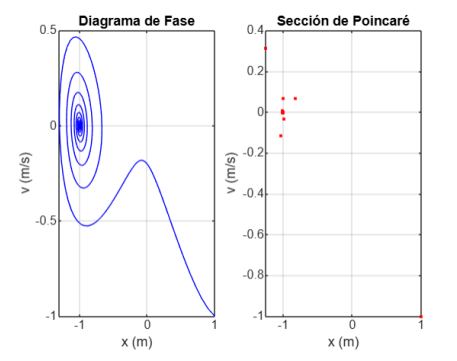
\includegraphics[width=0.75\textwidth]{g10.png}
    \caption{Diagrama de fase (izquierda) y sección de Poincaré (derecha) del oscilador amortiguado $\ddot{x} = x - x^3 - c\dot{x}$. Se observa la convergencia espiral hacia los puntos fijos estables.}
    \label{fig:seccion_poincare_oscilador_amortiguado} 
\end{figure}

\vspace{0.5cm}

\textbf{Conclusiones generales de la sección de Poincaré:}

\begin{itemize}
    \item \textbf{Sistema conservativo ($\ddot{x} = x - x^3$):} Presenta dinámica oscilatoria periódica con periodo dependiente de la amplitud. La sección de Poincaré muestra puntos discretos que confirman las órbitas cerradas del espacio de fases.
    
    \item \textbf{Sistema no conservativo ($\ddot{x} = x - x^3 - c\dot{x}$):} El amortiguamiento introduce disipación de energía, transformando las órbitas cerradas en espirales convergentes hacia los puntos fijos estables $(\pm 1, 0)$.
    
    \item \textbf{Técnica de análisis:} Las secciones de Poincaré permiten caracterizar la naturaleza del movimiento (periódico, cuasiperiódico o caótico) mediante la observación de la estructura de puntos en el espacio de fases reducido.
    
    \item \textbf{Importancia física:} La comparación entre ambos sistemas demuestra cómo los términos disipativos modifican fundamentalmente la topología del espacio de fases y la dinámica a largo plazo.
\end{itemize}

\newpage

\section{Autómata Celular 1D}

\subsection{Problema 1}
\subsubsection{Enunciado}
Implementar un autómata celular unidimensional con las siguientes especificaciones:

\begin{itemize}
    \item Utilizar la Regla 110 para la evolución del autómata
    \item Implementar dos condiciones iniciales independientes: una en la parte superior y otra en la parte intermedia
    \item Visualizar el resultado en forma de cruz sobre una matriz de células
    \item Las dimensiones y tamaños pueden definirse a criterio del implementador
\end{itemize}

\begin{figure}[H]
    \centering
    
\includegraphics[width=0.75\textwidth]{g11.png}
    \caption{Estructura objetivo para la visualización del autómata celular en forma de cruz}
    \label{fig:automata_objetivo}
\end{figure}

\subsubsection{Desarrollo}

\textbf{Fundamentos teóricos:}

Los autómatas celulares son sistemas dinámicos discretos donde cada celda evoluciona según reglas simples basadas en el estado de sus vecinos. La Regla 110 es una de las más estudiadas debido a su capacidad de generar patrones complejos y exhibir universalidad computacional.

\begin{figure}[H]
    \centering
    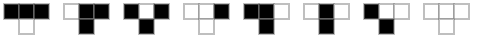
\includegraphics[width=0.5\textwidth]{g12.png}
    \caption{Tabla de transición de la Regla 110 del autómata celular unidimensional}
    \label{fig:regla_110}
\end{figure}

\textbf{Características de la Regla 110:}
\begin{itemize}
    \item Examina configuraciones de 3 células: izquierda, centro, derecha
    \item Cada configuración produce un nuevo estado según la tabla de transición
    \item Es Turing-completa, capaz de computación universal
    \item Genera patrones fractales y estructuras emergentes complejas
\end{itemize}

\textbf{Implementación:}

Se implementa un autómata celular con Regla 110 que presenta dos condiciones iniciales independientes en una matriz de 150×150 celdas. La visualización se restringe a una forma de cruz para mostrar las evoluciones de manera clara y estructurada.

\begin{lstlisting}[language=Octave, breaklines=true]
clear; clf; hold off;

% Parametros del automata
c = 150;                    % Tamano de la matriz
mitad = 75;                 % Punto de division para segunda condicion inicial

% Configurar visualizacion
figure;
axis([0 c 0 c]);
set(gca, 'xtick', [], 'ytick', []);
title('Automata Celular - Regla 110 (Visualizacion en Cruz)');

% Inicializacion de estructuras
acel = zeros(1, c);         % Vector estado actual
bcel = zeros(1, c);         % Vector estado siguiente  
mcel = zeros(c, c);         % Matriz completa de evolucion

% Funcion para aplicar Regla 110
function nuevo_estado = aplicar_regla110(izq, centro, der)
    patron = izq * 4 + centro * 2 + der;
    % Regla 110: 01101110 (binario) = 110 (decimal)
    regla = [0, 1, 1, 1, 0, 1, 1, 0];  % Indices 0-7
    nuevo_estado = regla(patron + 1);   % +1 para indexing de Octave
end

% FASE 1: Primera condicion inicial y evolucion (filas 1-75)
for i = 1:c
    acel(i) = round(rand);              % Generar primera fila aleatoria
end

for j = 1:mitad
    mcel(j, :) = acel;                  % Almacenar generacion actual
    
    % Calcular proxima generacion
    for i = 1:c
        izq = acel(mod(i-2, c) + 1);    % Vecino izquierdo (circular)
        centro = acel(i);               % Celula central
        der = acel(mod(i, c) + 1);      % Vecino derecho (circular)
        
        bcel(i) = aplicar_regla110(izq, centro, der);
    end
    
    acel = bcel;                        % Actualizar para siguiente iteracion
end

% FASE 2: Segunda condicion inicial y evolucion (filas 76-150)
for i = 1:c
    acel(i) = round(rand);              % Nueva fila aleatoria independiente
end

for j = (mitad + 1):c
    mcel(j, :) = acel;                  % Almacenar generacion actual
    
    % Calcular proxima generacion
    for i = 1:c
        izq = acel(mod(i-2, c) + 1);    % Vecino izquierdo (circular)
        centro = acel(i);               % Celula central
        der = acel(mod(i, c) + 1);      % Vecino derecho (circular)
        
        bcel(i) = aplicar_regla110(izq, centro, der);
    end
    
    acel = bcel;                        % Actualizar para siguiente iteracion
end

% FASE 3: Visualizacion en forma de cruz
hold on;
for j = 1:c
    for k = 1:c
        % Definir regiones de la cruz
        en_cabeza = (j >= 1 && j <= 50 && k >= 50 && k <= 100);
        en_brazos = (j >= 51 && j <= 100 && k >= 1 && k <= 150);
        en_base = (j >= 101 && j <= 150 && k >= 50 && k <= 100);
        
        % Dibujar celulas activas en la cruz
        if (en_cabeza || en_brazos || en_base) && mcel(j, k) == 1
            plot(k, c - j + 1, '.k', 'MarkerSize', 2);
        end
    end
end
\end{lstlisting}


\subsubsection{Análisis del algoritmo}

El algoritmo se estructura en tres fases principales:

\textbf{FASE 1: Primera evolución (filas 1-75)}
\begin{itemize}
    \item Genera una condición inicial aleatoria con distribución uniforme
    \item Aplica la Regla 110 iterativamente para 75 generaciones
    \item Utiliza fronteras circulares para manejar los bordes
\end{itemize}

\textbf{FASE 2: Segunda evolución (filas 76-150)}
\begin{itemize}
    \item Reinicia con una nueva condición inicial independiente
    \item Continúa la evolución por otras 75 generaciones
    \item Permite observar diferentes dinámicas emergentes
\end{itemize}

\textbf{FASE 3: Visualización selectiva}
\begin{itemize}
    \item Filtra las células según la geometría de cruz definida
    \item Divide la visualización en tres regiones: cabeza, brazos y base
    \item Solo muestra células activas (estado 1) dentro de la cruz
\end{itemize}

\textbf{Regla 110}

La Regla 110 examina cada celda y sus dos vecinos, aplicando la siguiente tabla:

\begin{center}
\begin{tabular}{|c|c|c|c|c|c|c|c|c|}
\hline
\textbf{Patrón} & 111 & 110 & 101 & 100 & 011 & 010 & 001 & 000 \\
\hline
\textbf{Resultado} & 0 & 1 & 1 & 0 & 1 & 1 & 1 & 0 \\
\hline
\end{tabular}
\end{center}

\textbf{Características técnicas del sistema:}
\begin{itemize}
    \item \textbf{Dimensión:} Matriz de 150×150 celdas
    \item \textbf{Topología:} Fronteras circulares (toro unidimensional)
    \item \textbf{Estados:} Binarios (0: inactivo, 1: activo)
    \item \textbf{Vecindario:} Moore de radio 1 (3 células)
    \item \textbf{Condiciones iniciales:} Dos distribuciones aleatorias independientes
\end{itemize}

Los resultados se muestran en la siguiente figura:

\begin{figure}[H]
    \centering
    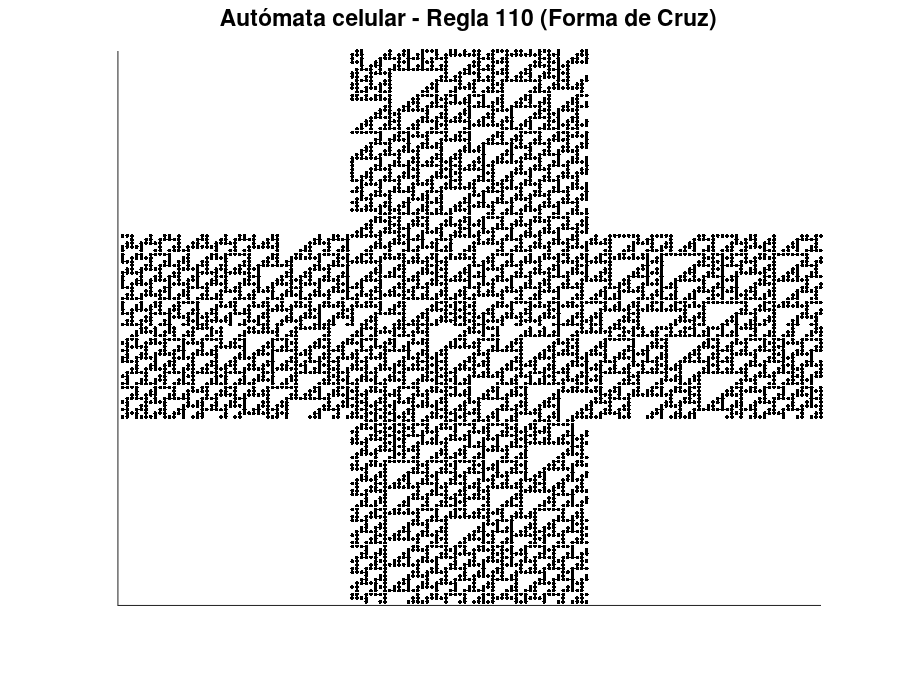
\includegraphics[width=0.8\textwidth]{g13.png}
    \caption{Visualización de la evolución del autómata celular Regla 110 en forma de cruz. Se observan dos patrones evolutivos distintos separados en la fila 76.}
    \label{fig:automata_resultado}
\end{figure}

\subsubsection{Conclusiones}

La implementación del autómata celular Regla 110 demuestra varios aspectos fundamentales:

\begin{itemize}
    \item \textbf{Emergencia de patrones:} A partir de condiciones iniciales aleatorias simples, surgen estructuras organizadas y patrones reconocibles
    
    \item \textbf{Sensibilidad a condiciones iniciales:} Las dos evoluciones independientes muestran dinámicas completamente diferentes, evidenciando la dependencia crítica de las condiciones iniciales
    
    \item \textbf{Universalidad computacional:} La Regla 110 es Turing-completa, capaz de realizar cualquier cálculo computable dado tiempo y espacio suficientes
    
    \item \textbf{Visualización estructurada:} La forma de cruz permite observar claramente la transición entre las dos evoluciones y los patrones emergentes en cada región
\end{itemize}

Entonces se puede ver cómo sistemas simples con reglas locales pueden generar comportamientos globales complejos, siendo un ejemplo paradigmático de los sistemas complejos y la computación emergente.



\end{document}


